%!TEX root = Main.tex
\documentclass[Main]{subfiles}

\begin{document}

\section{System Description} % (fold)
\label{sec:system_description}

	This section describes the system from a structural and a behavioural perspective, using SysML.
	For the structural description, a Block Definition Diagram and a Internal Block Diagram are used. For the behavioural perspective, a Activity Diagram is used.
	
	\subsection{Structure} % (fold)
	\label{sub:system_structure}

		The structural description is used to describe what parts the system is composed of, and how the parts communicate with each other.
		To depict this, a System Block Diagram is used to show composition, and a Internal Block Diagram is used to show dataflow. 
		These can be seen in \ref{fig:systembdd} and \ref{fig:systemibd}.
		
		\begin{figure}[H]
			\centering
			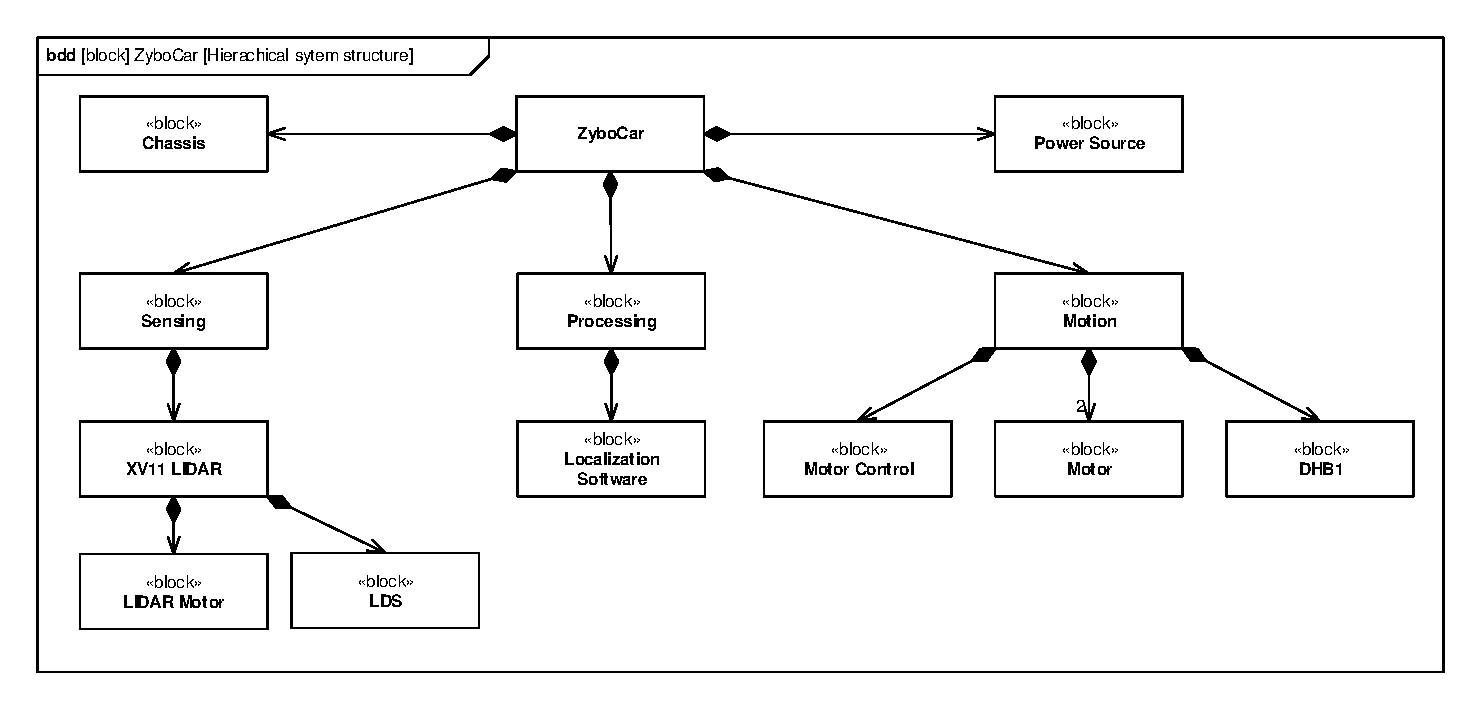
\includegraphics[width=\linewidth]{SystemBDD}
			\caption{System Block Diagram}
			\label{fig:systembdd}
		\end{figure}
		
		\begin{figure}[H]
			\centering
			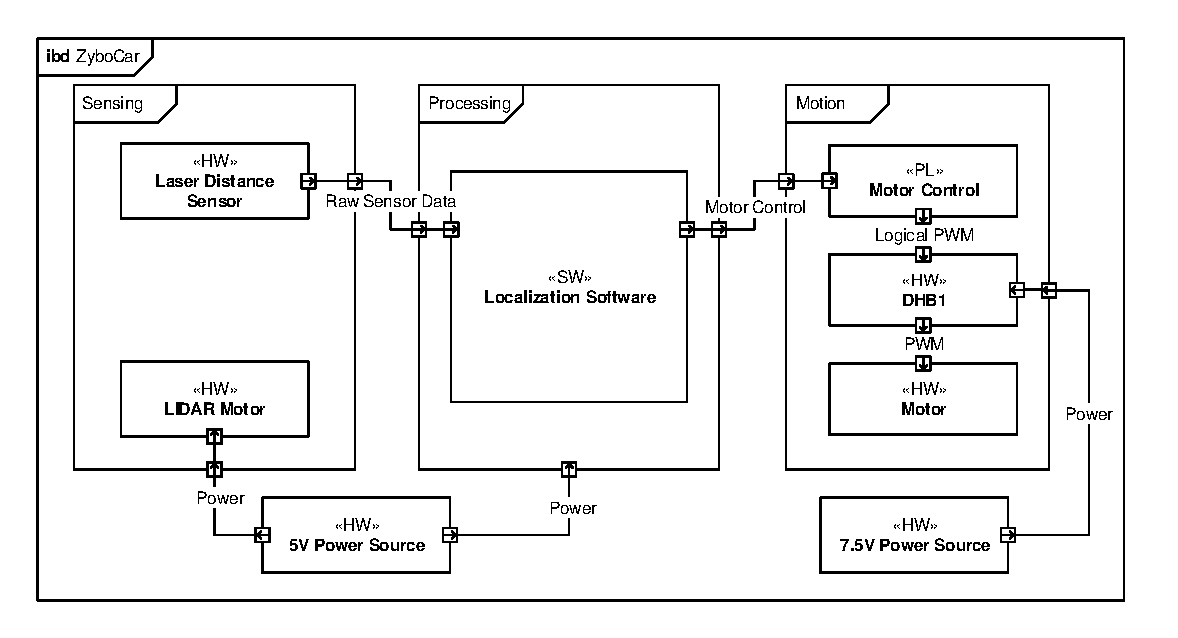
\includegraphics[width=\linewidth]{SystemIBD}
			\caption{System Internal Block Diagram}
			\label{fig:systemibd}
		\end{figure}
		
		In \ref{fig:systembdd} the main blocks of the system are shown. 
		The central block is the ZyboCar, which all other blocks are composed of.
		The sensing block contains the XV11 LIDAR, which is the sensor used for measuring distance at 360\degree.
		This raw sensing data is transferred to the processing block, which uses the sensor data to construct the next control signal for the motor block.
		The motion block contains a motor controller, two motors, and a Dual H-Bridge block.
		When the motor block receives a control signal from the localisation software, the motion controller converts the signal to a logical PWM signal, which the DHB then converts to a analoge PWM signal that can be used to control the Motor.
		
	\subsection{Behaviour} % (fold)
	\label{sub:system_behaviour}
		
		The behavioural description is used to describe what the system should do.
		At the behavioural level, composition is abstracted away. 
		Instead, emphasis is put on what actions should be made, what order they should be made in, and what input and output should come from each action.
		To depict this, a Activity Diagram is used. This can be seen in \ref{fig:systemact}.
		
		\begin{figure}[H]
			\centering
			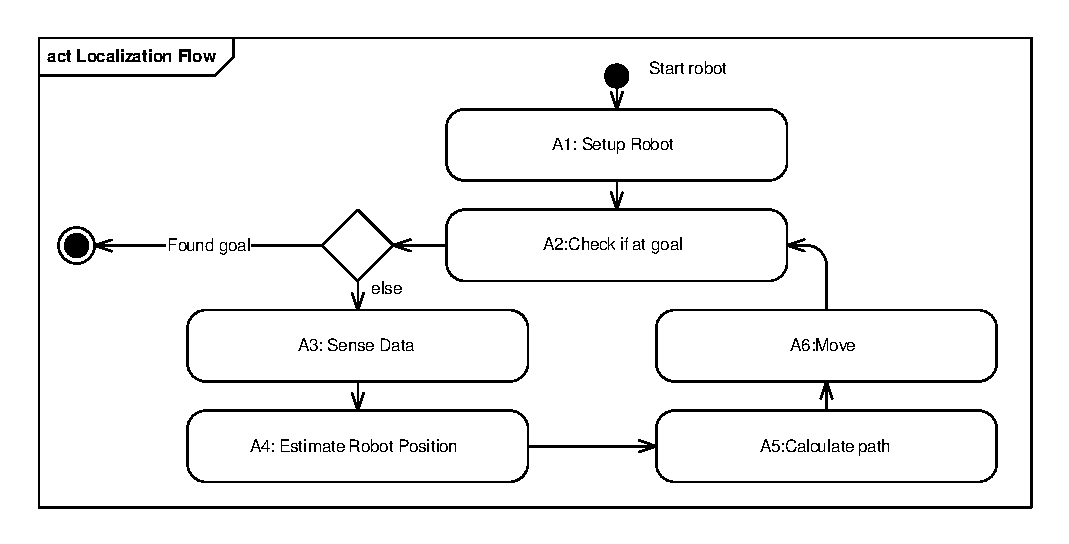
\includegraphics[width=\linewidth]{SystemACT}
			\caption{System Activity Diagram}
			\label{fig:systemact}
		\end{figure}
		
		The system starts by setting up the robot, and it then enters a loop that continues until the goal is found.
		
		When the robot has not yet found its goal, it starts out by using its sensor.
		Then it uses the sensordata to update the weights of its particles, and resample them.
		
		Using the resampled particels, the robots calculates its most probable current location.
		With basis in this location, a path to the goal is generated.
		Finally, the robot moves a step along the found path, and checks if it has reached the goal.


% section system_description (end)
\end{document}